\documentclass[11pt,a4paper]{report}
\usepackage[left=2cm,right=2cm,bottom=2cm,top=2cm]{geometry}
\usepackage[T1]{fontenc}     
\usepackage[utf8]{inputenc}  % Accents codés dans la fonte
\usepackage[frenchb]{babel}  % Les traductions françaises
\usepackage{hyperref}

\usepackage{numprint} %formate les chiffre par ex 1200 devient 1 200
\usepackage{csquotes}
\usepackage{listings} %env pour ecrire le code dans le document
\usepackage{color} %coloration du document
\usepackage{fancyhdr, graphicx, caption, subfig, wrapfig, enumitem} %pour les figures et logos du document
\graphicspath{{Pictures/}} % Specifies the directory where pictures are stored

\usepackage{datetime}
\newdate{date}{06}{02}{2017}

%format de l'env de code
\lstset{language=C}  % Set your language (you can change the language for each code-block optionally)
\definecolor{mygreen}{rgb}{0,0.6,0}
\definecolor{mygray}{rgb}{0.5,0.5,0.5}
\definecolor{mymauve}{rgb}{0.58,0,0.82}
\definecolor{mygrey}{rgb}{0.94,0.94,0.94}
\lstset{
  backgroundcolor=\color{mygrey},   % choose the background color
  basicstyle=\footnotesize,        % size of fonts used for the code
  breaklines=true,                 % automatic line breaking only at whitespace
  captionpos=b,                    % sets the caption-position to bottom
  commentstyle=\color{mygreen},    % comment style
  escapeinside={\%*}{*)},          % if you want to add LaTeX within your code
  keywordstyle=\color{blue},       % keyword style
  stringstyle=\color{red},	       % string literal style
  inputencoding=utf8,
  extendedchars=true,
  literate={à}{{\`a}}1 
  {è}{{\`e}}1 
  {é}{{\'e}}1 
  {ù}{{\`u}}1
  {ç}{{\c c}}1
  {ê}{{\^e}}1
  {'}{{\textquoteright}}1,
 }

\hypersetup{
	pdfauthor = {Herat Clement,Magni Paulu-Micheli},
	pdftitle = {Programmation C - Projet MasterMind},
	pdfsubject = {Compte Rendu de Projet},
	pdfkeywords = {arduino, C, MasterMind, EISC, Herat, Magni, LCD},
    pdfstartview={FitW}}



%debut du document
\begin{document}

\begin{titlepage} \begin{center}

    \begin{minipage}{0.48\textwidth} \begin{flushleft}
		
\includegraphics[height=0.12\textheight]{./logoEISC}
    \end{flushleft}\end{minipage}
    \begin{minipage}{0.48\textwidth} \begin{flushright}
		
\includegraphics[height=0.12\textheight]{./logoEsipe}
    \end{flushright}\end{minipage}
    
    \textsc{\huge{\textbf{ESIPE-MLV}}}\\
    \vspace{5mm}
    \textsc{\LARGE{\textbf{\'E}lectronique et \textbf{I}nformatique: \\ 
    			\textbf{S}ystèmes \textbf{C}ommunicants}} 

	\vfill
		\textsc{\LARGE Compte Rendu}
	\vfill
	    \underline {EISC-1}    
    \vfill
	
    \hrule \vfill
		{\huge \bfseries \textsc Projet Mini MasterMind }
    \vfill \hrule
    
    \vfill
    \begin{minipage}{0.48\textwidth} \begin{flushleft} \large
        \emph{Auteurs:}\\	
        \textsc{Hérat} Clément\\
        \textsc{Magni} Paulu-Micheli
	\end{flushleft}	\end{minipage}
    \begin{minipage}{0.48\textwidth} \begin{flushright} \large
        \emph{Enseignants:}\\	
        \textsc{Lohier} Stéphane\\
        \textsc{Revuz} Dominique
	\end{flushright} \end{minipage}
    
    \vfill
    	\textbf{\Large{ TP Programmation C}}
    \vfill
    
	\large\displaydate{date}
\end{center} \end{titlepage}

\tableofcontents
\thispagestyle{empty}

\listoffigures
\thispagestyle{empty} \newpage \setcounter{page}{1}

\chapter*{Introduction}
\addcontentsline{toc}{chapter}{Introduction}
    
	Dans le cadre de nos cours de programmation en langage C, et de leurs application en Travaux Dirigés sur Arduino\footnotemark, nous avons du réaliser un MasterMind.

\begin{wrapfigure}{l}{60mm}
	\centering
    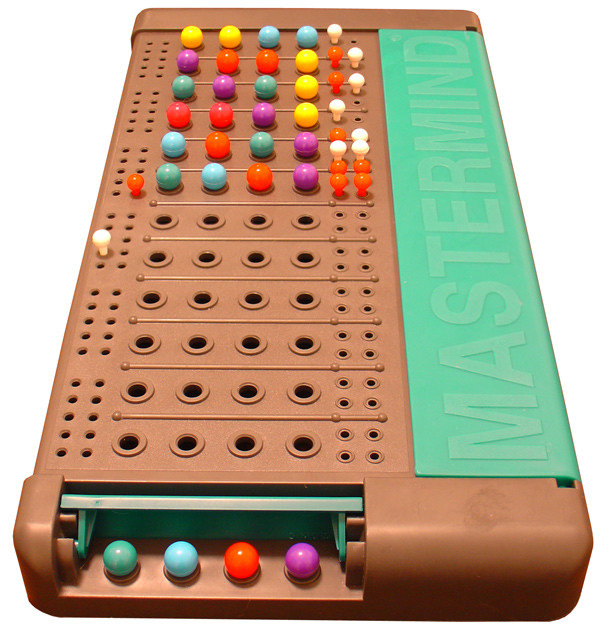
\includegraphics[height=60mm]{Mastermind.jpg}
    \captionof{figure}{Mastermind}
    \label{fig1}
\end{wrapfigure}
   	
    \paragraph{}
    Pour ceux qui ne connaissent pas, le MasterMind est un jeu de réflexion et de déduction qui se joue à deux. 
    Nous le trouvons généralement sous la forme de la figure\ref{fig1}.
\paragraph{}
    En voici donc le principe d'après \href{https://fr.wikipedia.org/wiki/Mastermind}{Wikipedia}:
	Un joueur commence par placer son choix de pions sans qu'ils soient vus de l'autre joueur à l'arrière d'un cache qui les masquera à la vue de celui-ci jusqu'à la fin de la manche.
	Le joueur qui n'a pas sélectionné les pions doit trouver quels sont les quatre pions, c'est-à-dire leurs couleurs et positions.

	Pour cela, à chaque tour, le joueur doit se servir de pions pour remplir une rangée selon l'idée qu'il se fait des pions dissimulés.
	Une fois les pions placés, l'autre joueur indique :
	\begin{enumerate}
		\item le nombre de pions de la bonne couleur bien placés en utilisant le même nombre de pions rouges.
		\item le nombre de pions de la bonne couleur, mais mal placés, avec les pions blancs.
	\end{enumerate}


\paragraph{}
	Il arrive donc surtout en début de partie qu'il ne fasse rien concrètement et qu'il n'ait à dire qu'aucun pion ne correspond, en couleur ou en couleur et position.
	La tactique du joueur actif consiste à sélectionner en fonction des coups précédents, couleurs et positions, de manière à obtenir le maximum d'informations de la réponse du partenaire puisque le nombre de propositions est limité par le nombre de rangées de trous du jeu. 
    
	Dans la plupart des cas, il s'efforce de se rapprocher le plus possible de la solution, compte tenu des réponses précédentes, mais il peut aussi former une combinaison dans le seul but de vérifier une partie des conclusions des coups précédents et de faire en conséquence la proposition la plus propice à la déduction d'une nouvelle information.

	Le joueur gagne cette manche s'il donne la bonne combinaison de pions sur la dernière rangée ou avant. Dans tous les cas, c'est à son tour de choisir les pions à découvrir. 
Mais il est interdit de mettre une couleur en double, en triple ou en quadruple aussi bien dans les pions secrets que dans les pions \og publics \fg.

\paragraph{}
Les objectifs de ce projet sont:
\begin{itemize}
	\item de développer des algorithmes.
    \item d'appliquer les connaissances théoriques acquises en cours de programmation de langage C.
    \item de travailler sur les entrées/sorties de la carte Arduino.
    \item de réaliser un montage électronique fonctionnel.
\end{itemize}

\footnotetext[1]{Arduino is an open-source electronics platform based on easy-to-use hardware and software. It's intended for anyone making interactive projects. \emph{\url{https://www.arduino.cc/}}}
\chapter{Montage de l’écran LCD}

\section{Présentation écran}
\begin{figure}[h]
	\centering
	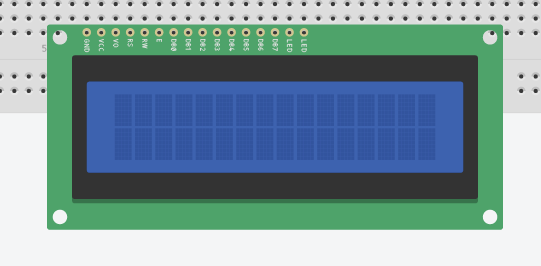
\includegraphics[width=0.5\linewidth]{lcd.png}
    \caption{Écran LCD}
    \label{lcd}
\end{figure}
Au cours de ce projet nous allons utiliser un écran LCD 16x2 équipé du driver Hitachi HD44780 (figure \ref{lcd}). Ce type d'écran est compatible avec la librairie \og LiquidCrystal \fg disponible nativement au sein de l'IDE\footnotemark Arduino 

%%
 \footnotetext[1]{IDE: Entegrated Eevelopment Environment ; ou EDI en français: Environnement de Développement Intégré.
 	source \href{https://en.wikipedia.org/wiki/Integrated_development_environment}{Wikipedia}}
%%

\begin{figure}[h]
	\centering
	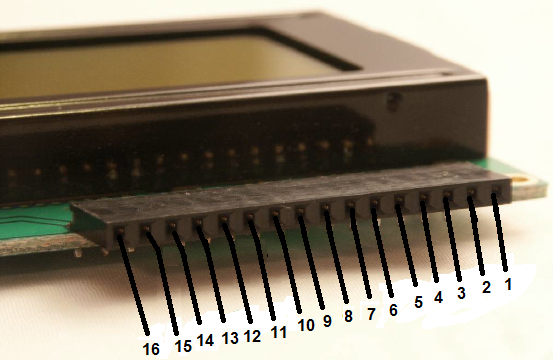
\includegraphics[width=12cm]{HD44780-LCD-pinout.png}
    \caption{Pin écran LCD}
    \label{PinLCD}    
\end{figure}


\paragraph{}
	Description des pins :
    \begin{enumerate}[label=\arabic*]
    	\item Vss - Masse 0V de l'écran LCD.
		\item Vcc - Pin d'alimentation de l'écran. Le voltage accepté est entre 3.3V et 5V.
		\item Pin d'ajustement du contraste. On y branche un potentiomètre pour faire varier le contraste.
		\item Pin sélection du registre. Si égale a 0 : mode commande, si égale a 1 : mode données.
		\item Pin de lecture/écriture. Si égale a 0 : mode écriture, si égale a 1 : mode lecture.
		\item Pin de validation.
		\item Bus de données, bit 0
		\item Bus de données, bit 1
		\item Bus de données, bit 2
		\item Bus de données, bit 3
		\item Bus de données, bit 4
		\item Bus de données, bit 5
		\item Bus de données, bit 6
		\item Bus de données, bit 7
		\item Alimentation du rétroéclairage de l'écran. La tension d'entré maximale est 5V et correspond a l'éclairage maximum. On peut y connecter un potentiomètre pour faire varier l'intensité du rétroéclairage.
		\item Pin de terre du rétroéclairage.
    \end{enumerate}
    
\newpage
\section{Montage}
\begin{figure}[h]
	\centering
	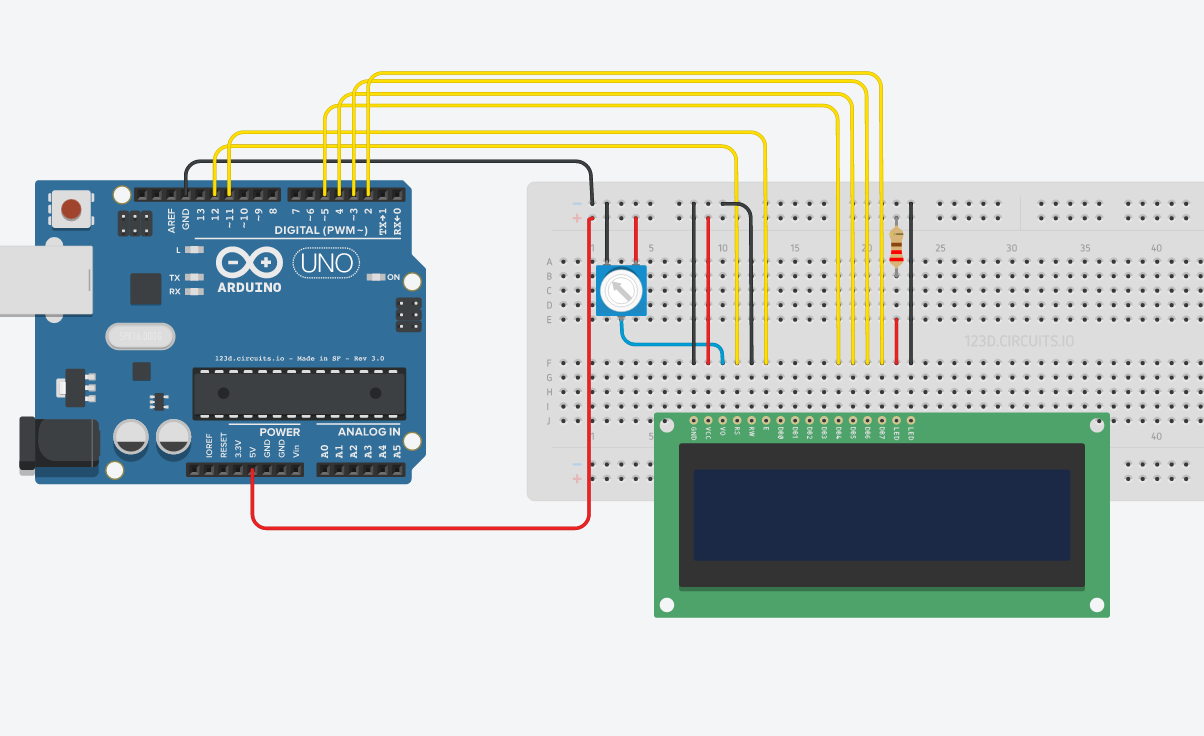
\includegraphics[width=\linewidth]{montageLCD.png}
    \caption{Montage écran LCD}
    \label{montageLCD}    
\end{figure}
Pour le montage de l'écran LCD et de l'Arduino (figure \ref{montageLCD}) nous avons utilisés :
\begin{itemize}
	\item 1 écran LCD,
    \item 1 potentiomètre $10k\Omega$,
    \item 1 Arduino Uno,
    \item 1 résistance $220\Omega$,
    \item 5 fil noir,
    \item 4 fil rouge,
    \item 1 fil bleu,
    \item 6 fil jaune.
\end{itemize}


\chapter{Ajout de deux boutons poussoirs}

\section{Montage des boutons}
Comme vous pouvez le voir sur la figure \ref{montageBoutons} nous avons montés les boutons en montage Pull-Down ainsi que évoqué sur la figure \ref{montagePullDown} sur les entrées 8 et 9 de l'Arduino.
\begin{figure}[h]
	\centering
	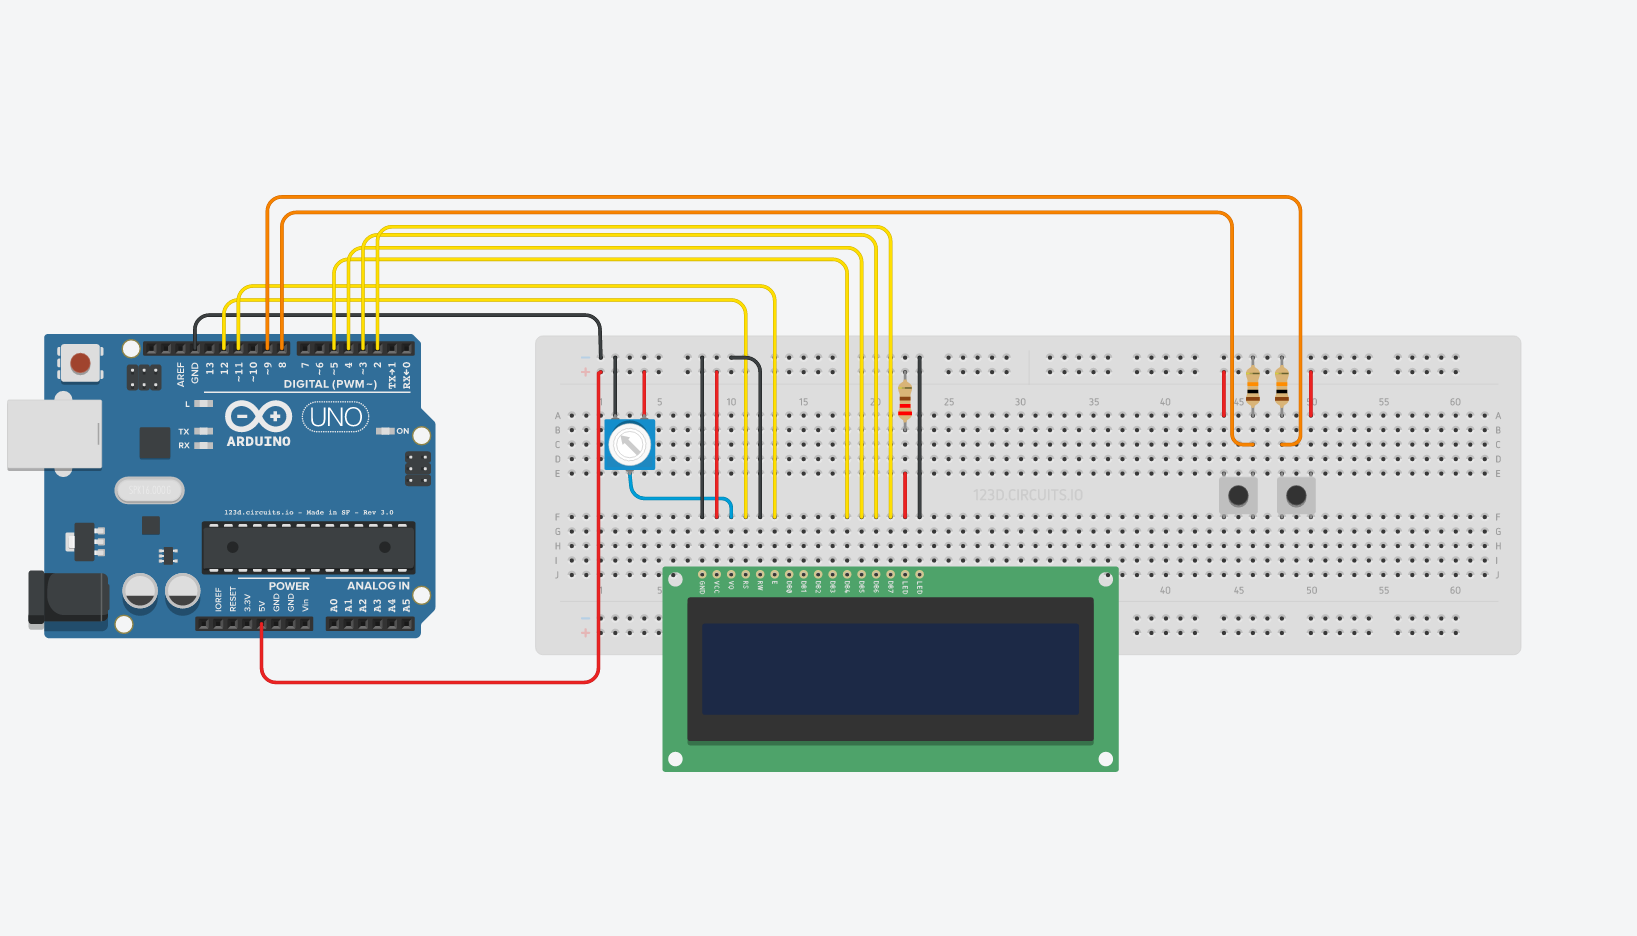
\includegraphics[width=\linewidth]{montageBouttons.png}
    \caption{Montage Boutons}
    \label{montageBoutons}    
\end{figure}

\newpage
\section{Montage Pull-Down}
\paragraph{}
	Nous pouvons remarquer sur le montage de la figure \ref{montageBoutons} deux résistance placées a la sortie des boutons poussoir. Il s'agit de résistance dites "Pull-Down". Ces resistance ont deux roles tres important, elles servent à assurer le bon fonctionnement du bouton, mais également la sécurité du circuit.
    
\begin{figure}[h]
	\centering
	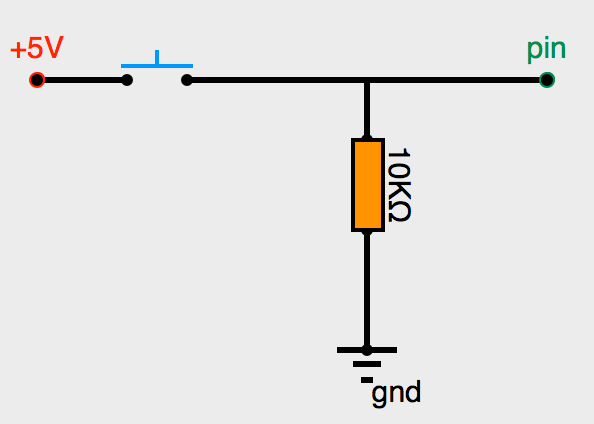
\includegraphics[width=10cm]{boutonPullDown.png}
    \caption{Montage d'une résistance en Pull-Down}
    \label{montagePullDown}
\end{figure}

\paragraph{}
	L'électricité choisis toujours le chemin le moins résistif. Mais si elle n'a pas le choix, elle passe tout de même là où ça résiste.

	Nous allons donc ajouter une résistance à notre circuit. Une assez forte pour que le courant ne passe que s'il y est obligé (ici de $10k\Omega$).
	Si le poussoir est baissé, le courant va du +5V a la pin de l'Arduino. Il ne prendra pas le chemin de la masse car la résistance lui demande un effort(Et dans le cas contraire la resistance protegera le montage d'un court-circuit). La pin de l'Arduino recevra du +5V et indiquera HIGH (ou 1).

	Si le poussoir est levé, donc le circuit ouvert, le très faible courant résiduel qui sortira du pin de l'Arduino sera absorbé par la masse, le pin sera donc bien en LOW (ou 0)



\newpage
\section{Programme}
\underline{Programme utilisé pour tester le bon fonctionnement de l'acquisition des boutons:}
\lstinputlisting[language=c]{Sources/testBoutons.ino}

\newpage
\paragraph{}
\underline{Voici les affichages obtenus:}
\begin{itemize}
	\item Lorsqu'on appuie sur aucun boutons:
    \begin{figure}[h]
    	\centering
        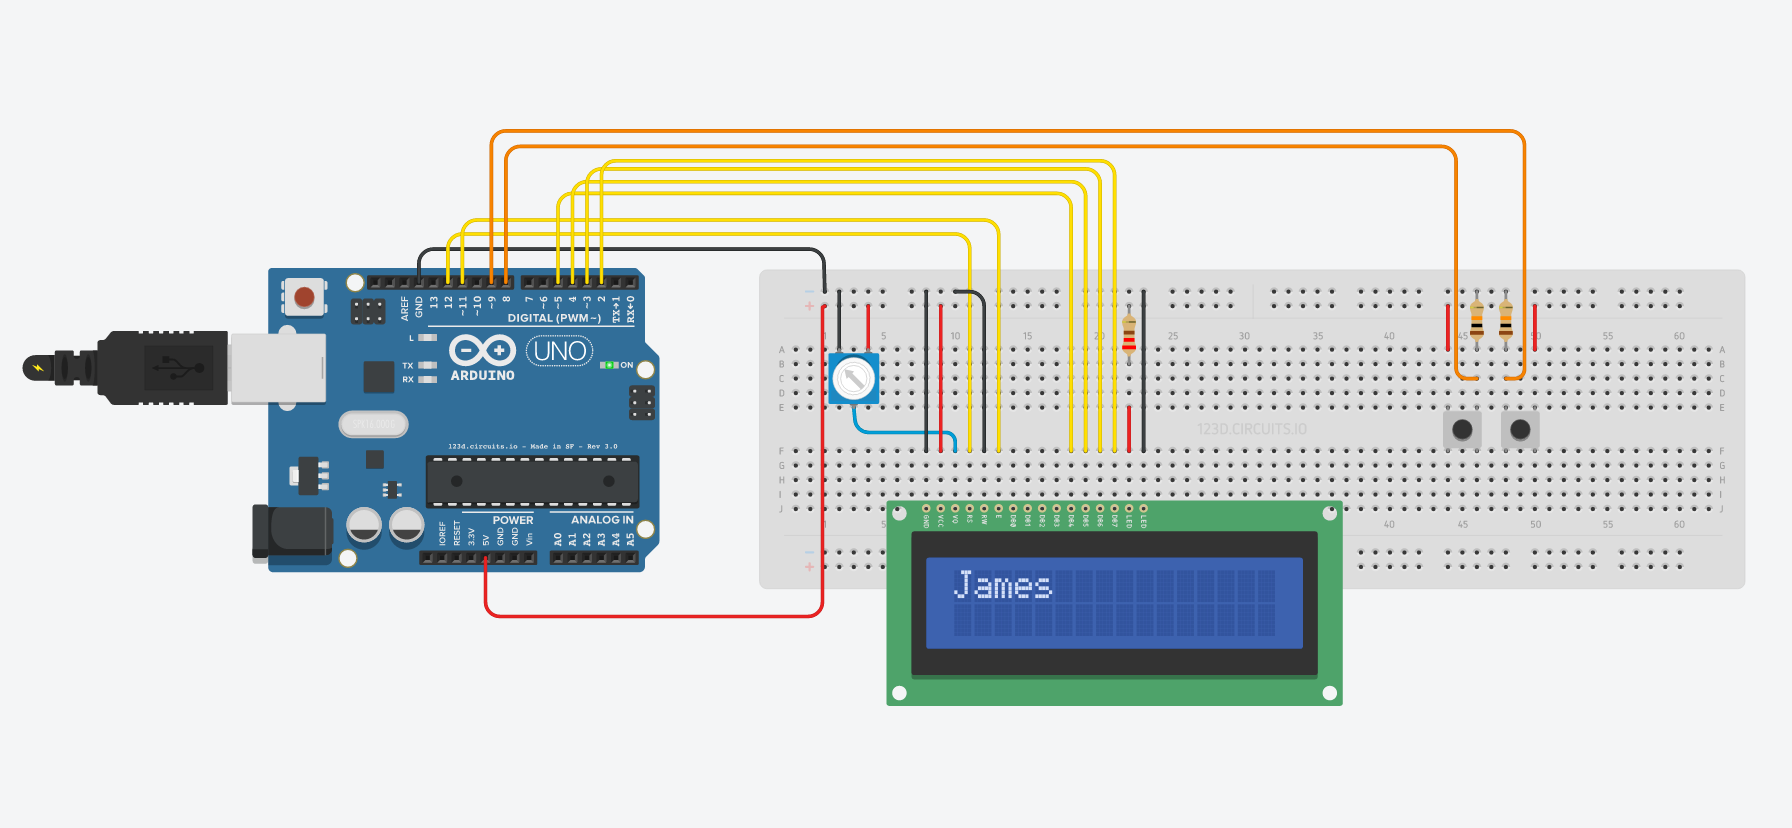
\includegraphics[width=\linewidth]{testbutons_0.png}
        \caption{Test sans appuyer sur les boutons}
        \label{testbutons0}
    \end{figure}
    
    \item Lorsqu'on appuie sur un des 2 boutons:
    \begin{figure}[h]
    	\centering
        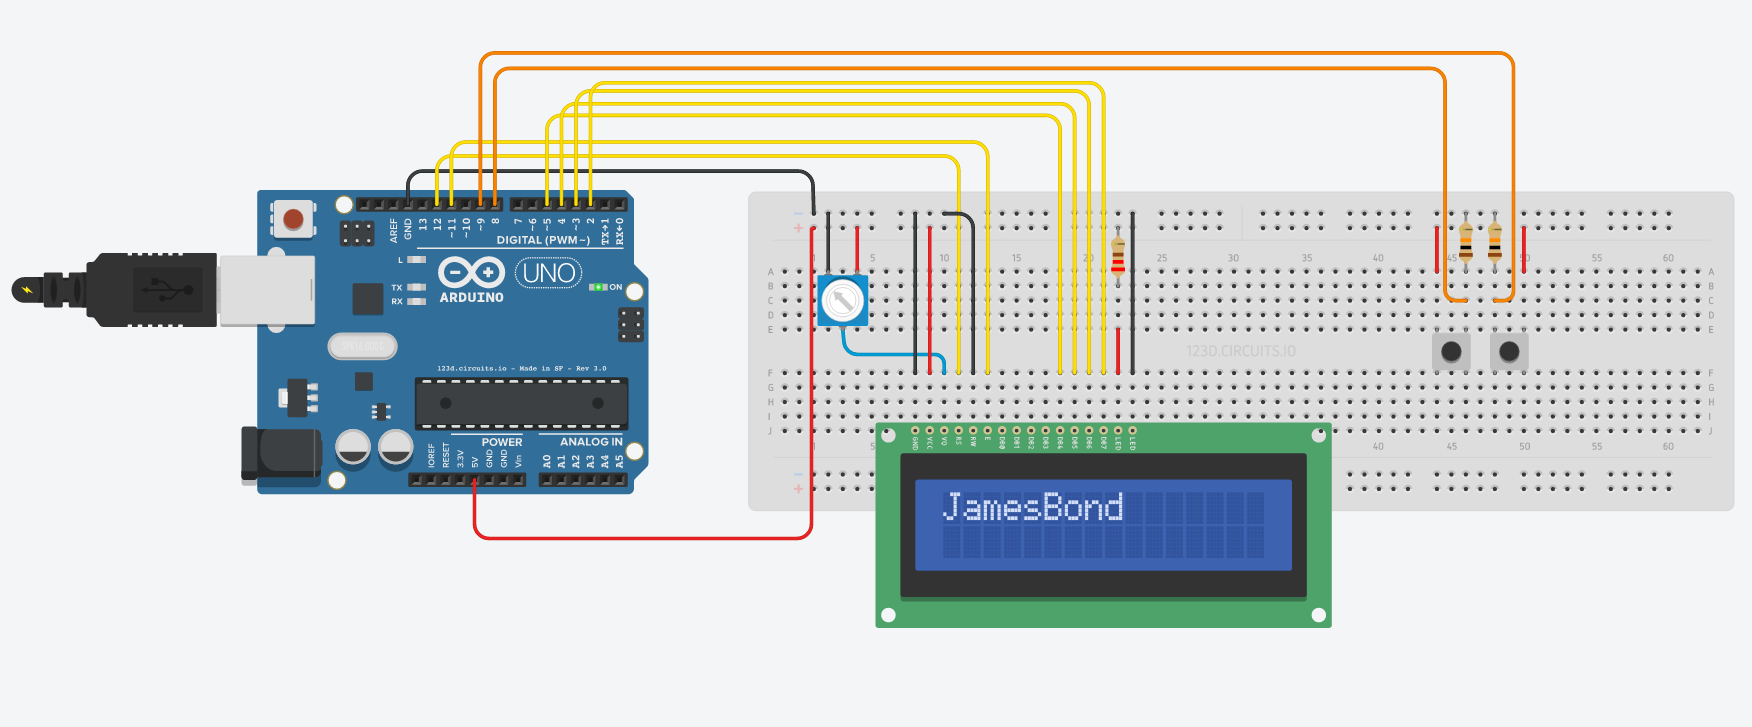
\includegraphics[width=\linewidth]{testbutons_1.png}
        \caption{Test en appuyant sur un des deux boutons}
        \label{testbutons1}
    \end{figure}
\end{itemize}


\chapter{Affichage et choix des caractères}

	Il faut maintenant réaliser une fonction pour l'affichage et le choix des caractères afin que le joueur puisse saisir une réponse.
    
	Il faut également que cette fonction stocke, de façon pertinente, la réponse du joueur afin qu'une autre fonction puisse en calculer le résultat.
    C'est à dire comparer sa réponse à la solution et dire combien de lettres sont bonnes mais mal positionnées et combien de lettres sont bonnes et bien placées.
	Et qu'entre deux réponses nous ayons la place d'afficher le résultat de la réponse précédente.

\section{Choix de l'algorithme}
	Pour réaliser cette fonction nous avons identifiés plusieurs solution lors de l'étude préalable du programme. 
    Nous avons donc choisi de réaliser une fonction qui enregistrera seulement la réponse actuellement en cours de saisie et qui utilisera la rémanence de l'écran pour conserver les réponses et résultats précédents.
    
    En effet précédemment nous avions remarqué que tant que l'écran n'était pas "nettoyé" l'affichage se conservait dans son état actuel.
    Cette solution simplifiait beaucoup le reste du programme et permettait de limiter les accès mémoire lors de la saisie des réponses et de l'affichage.

\section{Programme}
\underline{Programme utilisé pour tester la fonction de saisie: }
\lstinputlisting{Sources/TestSaisie.ino}

\newpage
\underline{Affichage obtenus lors du test de l'affichage et de la saisie des caractères:}
\begin{figure}[h]
	\centering
   	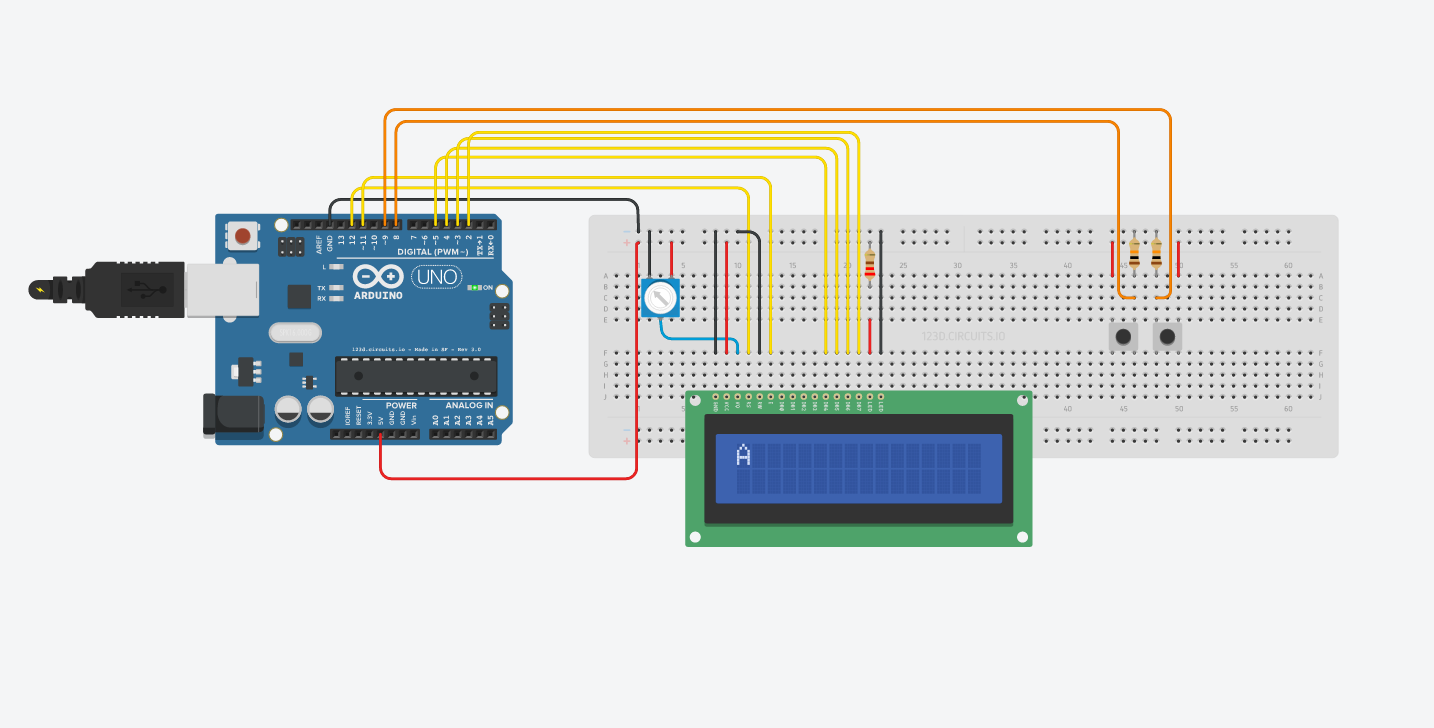
\includegraphics[width=\linewidth]{testSaisie1}
    \caption{Début de la saisie de la 1\iere{} réponse}
    \label{testSaisie1}
\end{figure}

\paragraph{}
Comme nous pouvons le voir sur la figure \ref{testSaisie2} l'affichage est conforme à nos attentes, nous avons bien un espace vide entre deux réponses ainsi qu'un saut a la ligne arrivé au bord de l'écran.
\begin{figure}[h]
	\centering
   	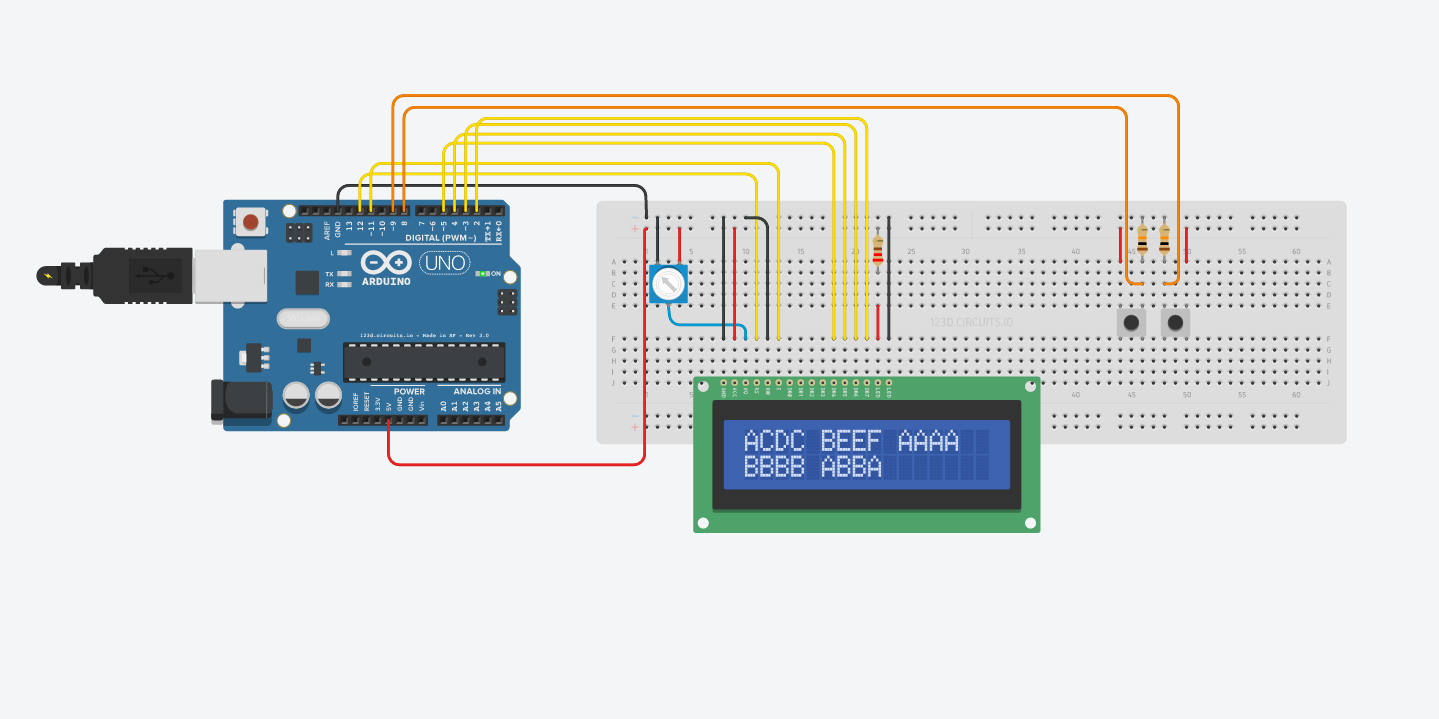
\includegraphics[width=\linewidth]{testSaisie2}
    \caption{Fin de la saisie de la 5\ieme{} réponse}
    \label{testSaisie2}
\end{figure}
\chapter{Calcul du résultat}
\paragraph{}
	Il faut maintenant réaliser une fonction de calcul du résultat.
Cette fonction devra a partir du code secret et de la réponse entrée par le joueur nous indiquer le nombre de lettres bien placées et le nombre de lettres mal placée.

\section{Algorithme}
\paragraph{}
	Pour cet algorithme il a fallut prendre en compte un point important : la possibilité d'avoir plusieurs fois la même lettre dans le code ou la réponse.
Un algorithme ne prenant pas cette information en compte pourrais entraîner des erreur.  

Prenons un exemple : 
  \begin{itemize}
    \item Code secret : "ABBA"
    \item Réponse : "ABCD"
  \end{itemize}
Dans ce cas un algorithme ne prenants pas en compte les double lettre pourrais considérer le A de la réponse comme étant a la fois a la bonne place mais aussi comme étant mal placé car "ABBA" contient deux 'A'.
Pour éviter cela nous avons du mettre en place un moyen de mémoriser les élément déjà identifier comme bien ou mal placés afin d'éviter le problème de double résultats.

	Nous avons donc décider de directement modifier les tableaux contenant le code secret et la réponse.\\
    
    Lorsque nous identifions deux lettres comme etant identique :
    \begin{itemize}
    \item La lettre du tableau code secret est passées en minuscules afin d'empecher une autre égalité lors de la comparaison sans perdre de donnée car il nous suffira simplement de repasser les lettres en majuscules pour revenir a l'etat initial
    \item La lettre du tableau reponse est mise a 1 ou 2 selon qu'elle soit bien placé ou non. La perte de donnée n'etant pas importante car nous ne reutilisons pas ces données par la suite. 
    \end{itemize}

\paragraph{}
Une fois cela pris en compte l'algorithme est assez simple et se deroule en trois étapes :
\begin{enumerate}
\item identification des lettres bien placées 
\item identification des lettres mal placées
\item mise en majuscule des lettres ayant été mise en minuscule
\end{enumerate}
 
 
\newpage
\section{Programme}
\underline{Programme utilisé pour calculer les résultats:}
\lstinputlisting[language=c]{Sources/GetAnswer.c}

\chapter{Affichage du résultat}
	Après avoir réaliser la fonction de calcul du résultat il convient d'en réaliser sa fonction d'affichage. 
    Nous avons trouvé que la méthode d'affichage en binaire proposée dans le cadre du projet n'était pas forcément des plus intuitive à comprendre.
    
    En conséquence nous en avons cherché une nouvelle plus facile à comprendre pour un néophyte.
    
\section{L'affichage retenu}
	Comme nous sommes sur un afficheur où chaque caractères est constitué de 5x8 pixels, nous avons choisi l'affichage que vous pouvez voir sur la figure \ref{affichagefull} avec sur la gauche autant de lignes que d'éléments bien placés et à droite autant de lignes que de bons éléments mais mal placés
    
  Pour davantage de facilités à lire et à implémenter également, nous avons disposés les lignes alternativement.
  
    \begin{figure}[h]
        \centering
        \subfloat[Affichage de toutes les possibilités]{\label{affichagefull}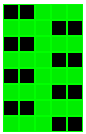
\includegraphics[width=3cm]{affichageResultatFull.png}}    
        \hspace{5pt}
        \subfloat[Dans le cas où on en a 3 bien placés et 1 mal placé]{\label{affichage32}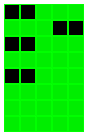
\includegraphics[width=3cm]{affichageResultat31.png}}
        \hspace{5pt}
        \subfloat[Dans le cas où on en a 0 de bien placés et 2 de mal placé]{\label{affichage02}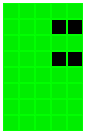
\includegraphics[width=3cm]{affichageResultat02.png}}
        
        \subfloat[En situation de jeu dans le cas ou la réponse secrète est DBAE]{\label{affichageEx}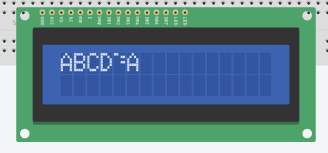
\includegraphics[height=4cm]{affichageResultEx.png}}
        \caption{Exemples de résultats obtenus}
        \label{affichages}
    \end{figure}

  
\section{Le programme}
	Pour parvenir au résultat ci-dessus nous avons utilisé la fonction \og createChar()\footnotemark \fg de la librairie LiquidCrystal.
	Pour faire un bref résumé, c'est une fonction qui permet de créer un caractère pixel par pixel.
    A cette fin il y a 8 caractères de la librairie qui sont disponible (de 0 à 8).
    Ceci est possible car dans la libraire LiquidCrystal les caractères sont sous la forme suivante:
  
  \begin{lstlisting}
byte smiley[8] = {
    B00000,
    B10001,
    B00000,
    B00000,
    B10001,
    B01110,
    B00000,
};
  \end{lstlisting}
  
  
  C'est un tableau de type byte ou chaque \og B***** \fg (byte) définit une ligne, chaque \og * \fg peut valoir 0 ou 1. 
  On peut donc éteindre ou allumer chaque pixels de chaque lignes indépendamment.
  
\paragraph{}
\underline{Programme d'affichage des résultats:}
\lstinputlisting{Sources/TestAffichage.ino}
    
\footnotetext {voir la page:\href{https://www.arduino.cc/en/Reference/LiquidCrystalCreateChar}{arduino.cc}}  
\chapter{Synthèse}

Dans cette version 2.1 du Mastermind vous trouverez des leds mais aussi des niveaux, cinq en tout (extrait du commentaire final du programme):
\begin{enumerate}
\item \emph{Beginner} : niveau débutant, "finger in the nose"
	\begin{itemize}
      \item Pas le droit à plusieurs fois la même lettre
      \item Les lettres possible sont de A à E
	\end{itemize}
    
\item \emph{Normal} : règles officielle du Mastermind
	\begin{itemize}
      \item Pas le droit à plusieurs fois la même lettre
      \item Les lettres possible sont de A à F
	\end{itemize}
    
\item \emph{Teacher} : règles demandées dans le sujet du projet
	\begin{itemize}
      \item Plusieurs même lettres possibles
      \item Les lettres possible sont de A à F
	\end{itemize}
    
\item \emph{Hard} : niveau difficile, "Good Luck !"
	\begin{itemize}
      \item Plusieurs même lettres possibles
      \item Les lettres possible sont de A à G
	\end{itemize}
    
\item \emph{42} : niveau solution 404 "Fuyez Pauvres Fous!"
	\begin{itemize}
      \item Plusieurs même lettres possibles
      \item Les lettres possible sont tout l'alphabet !!
	\end{itemize}
\end{enumerate}

\newpage
\section{Programme}
\underline{Code source du programme:}
\lstinputlisting{Sources/Mastermind.ino}

\newpage
\section{Quelques images de la version finale:}
\begin{figure}[h]
	\centering
		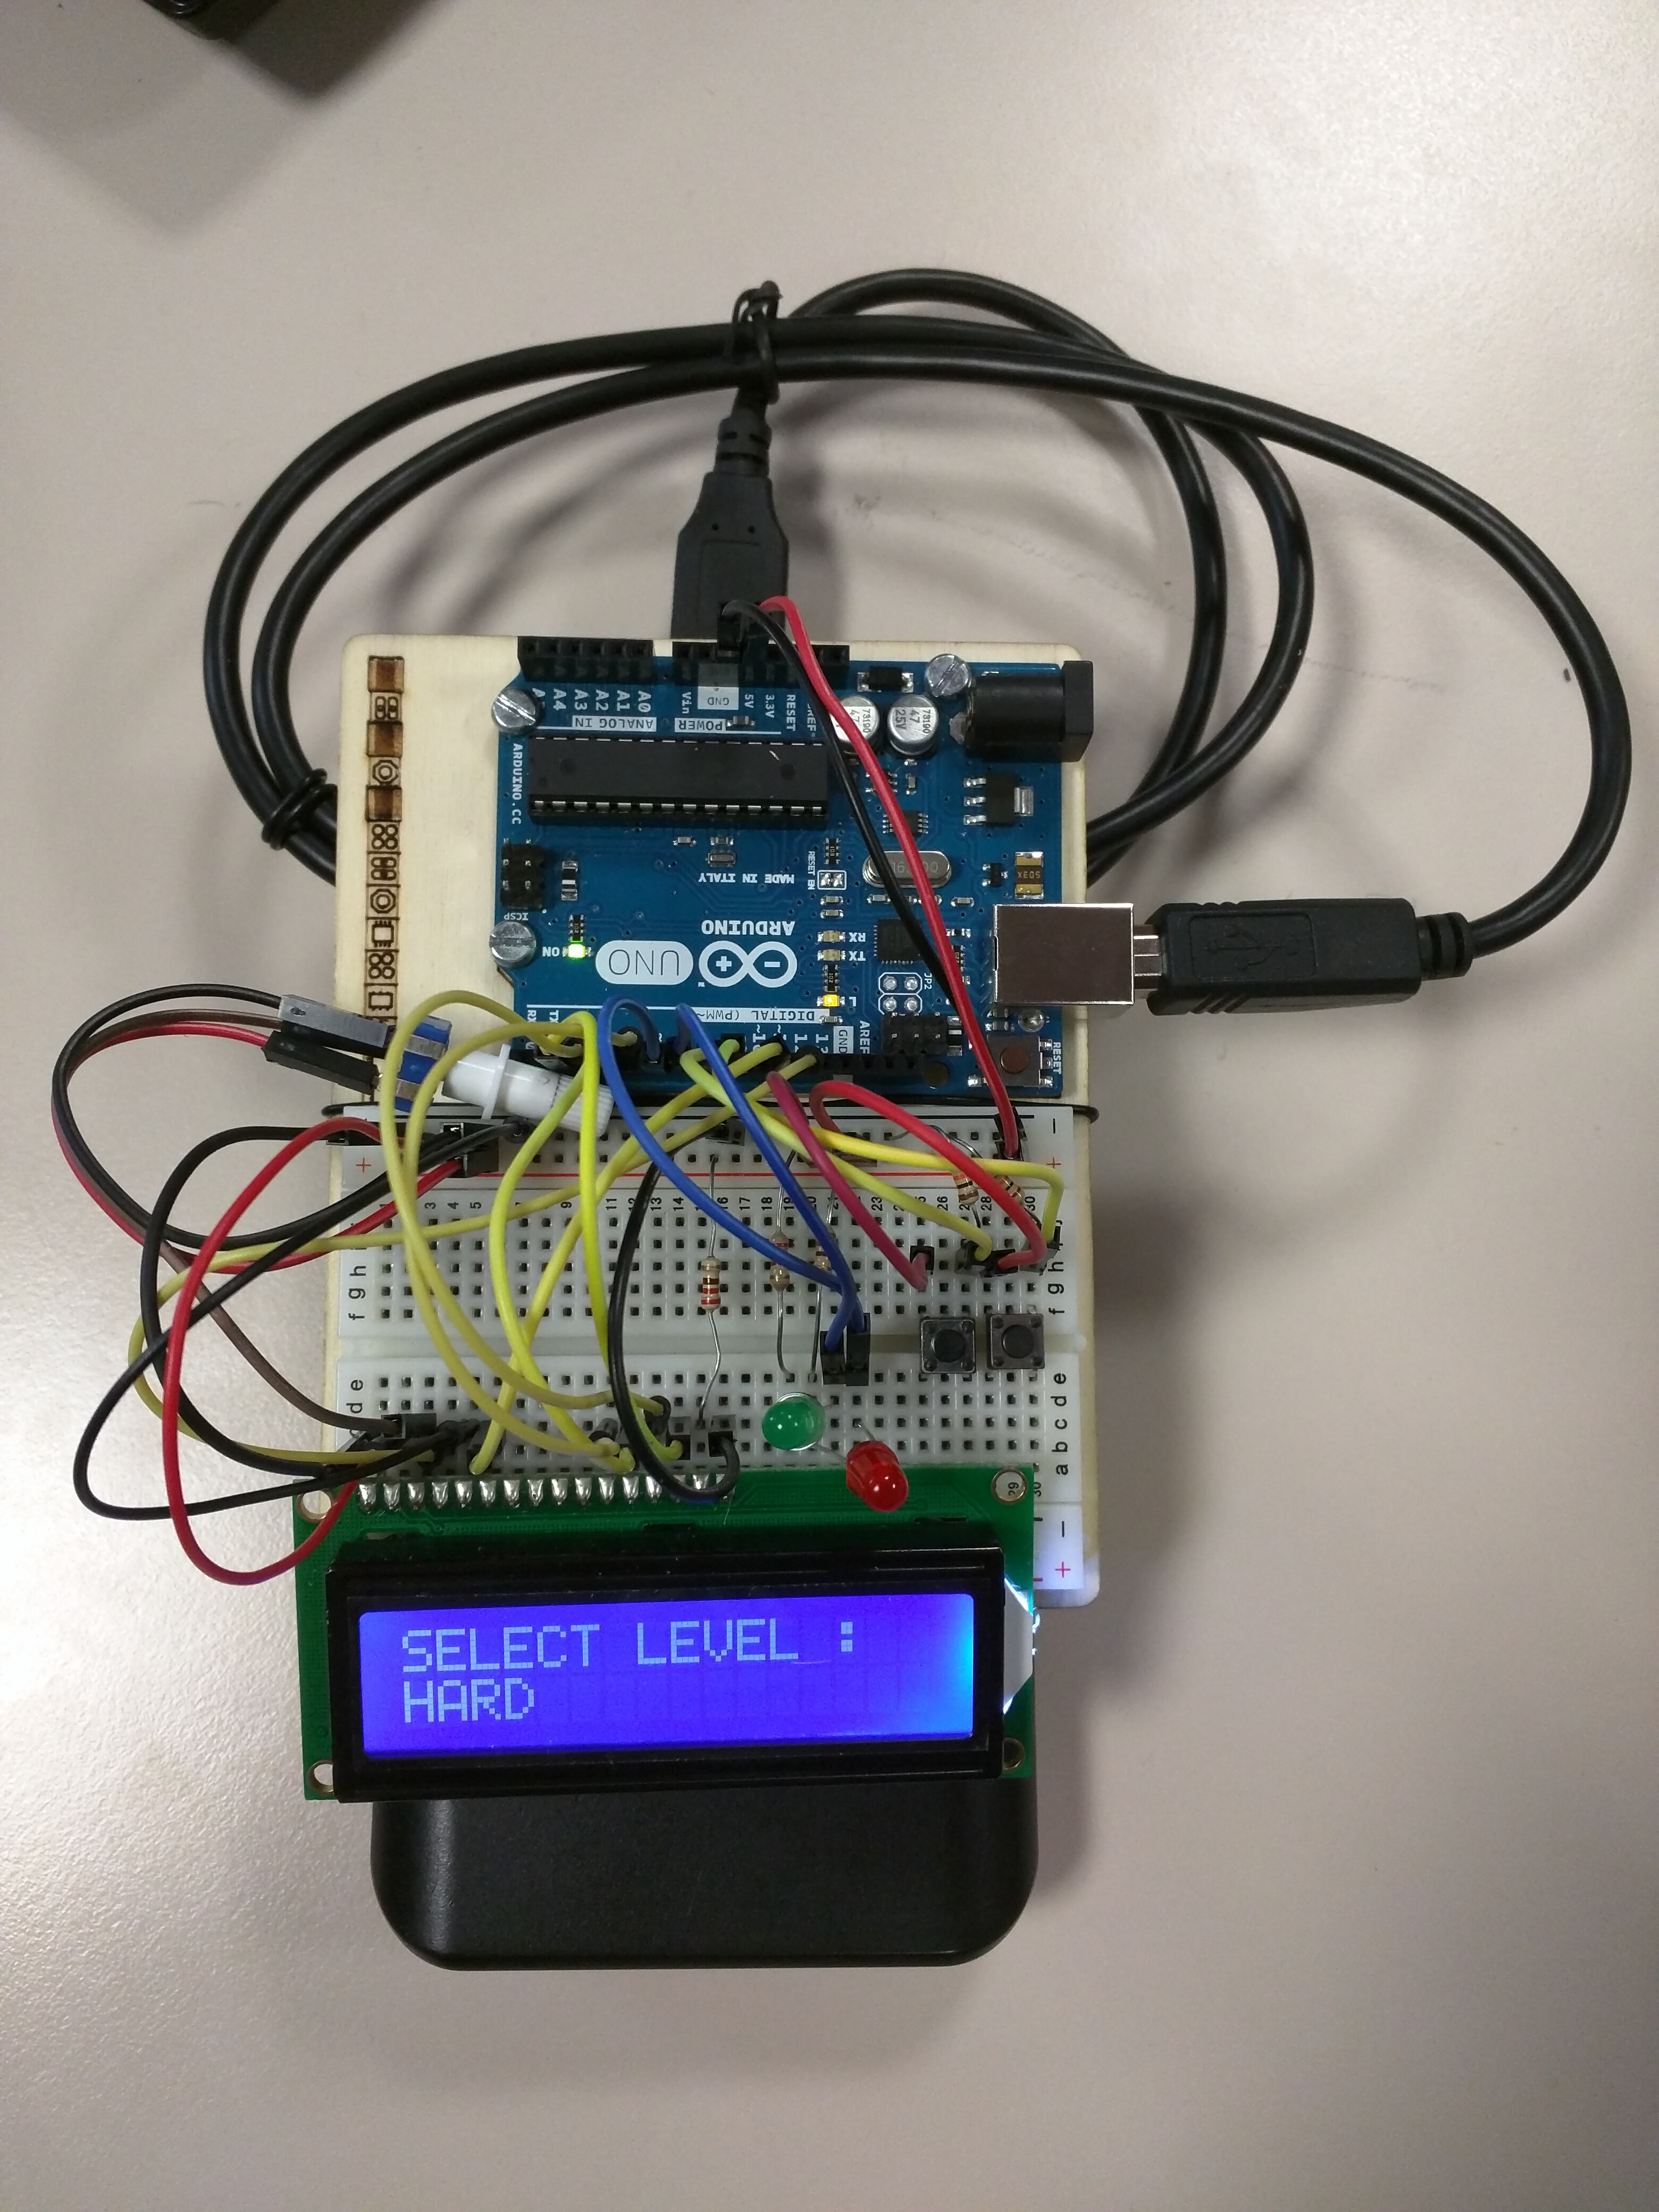
\includegraphics[height=18cm]{1.jpg}
        \caption{Montage final avec batterie pour pouvoir jouer partout}
\end{figure}

\begin{figure}[h]
	\centering
		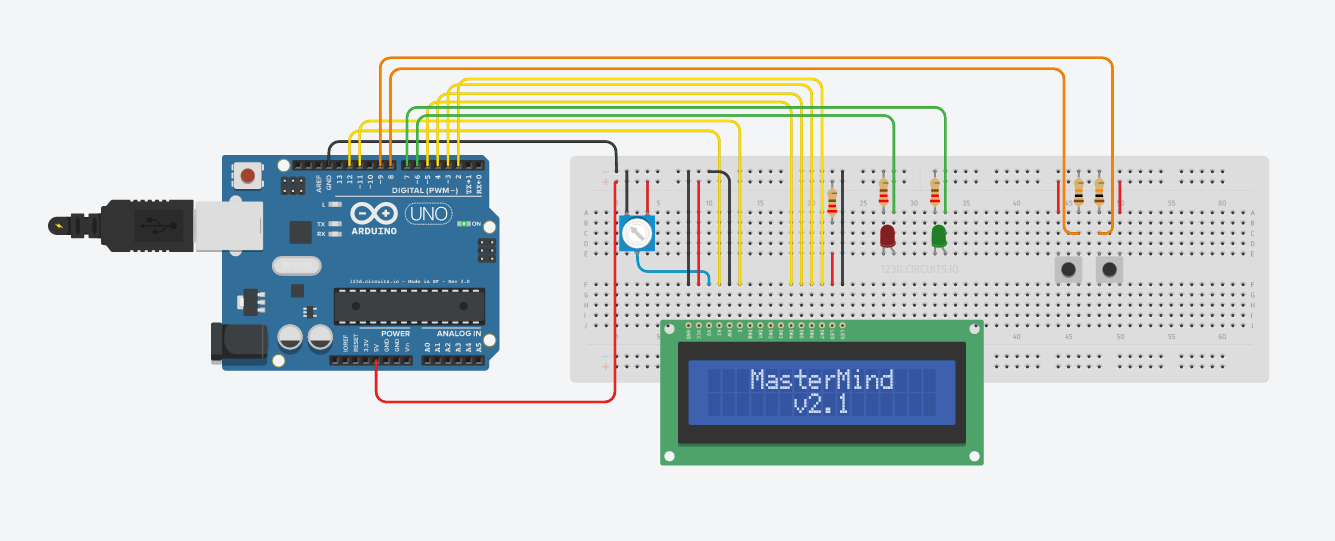
\includegraphics[width=\linewidth]{affichagefinal.png}
        \caption{Montage final du Projet Mastermind}
\end{figure}

\begin{figure}[h]
	\centering
      \subfloat[Début de partie]{\label{3}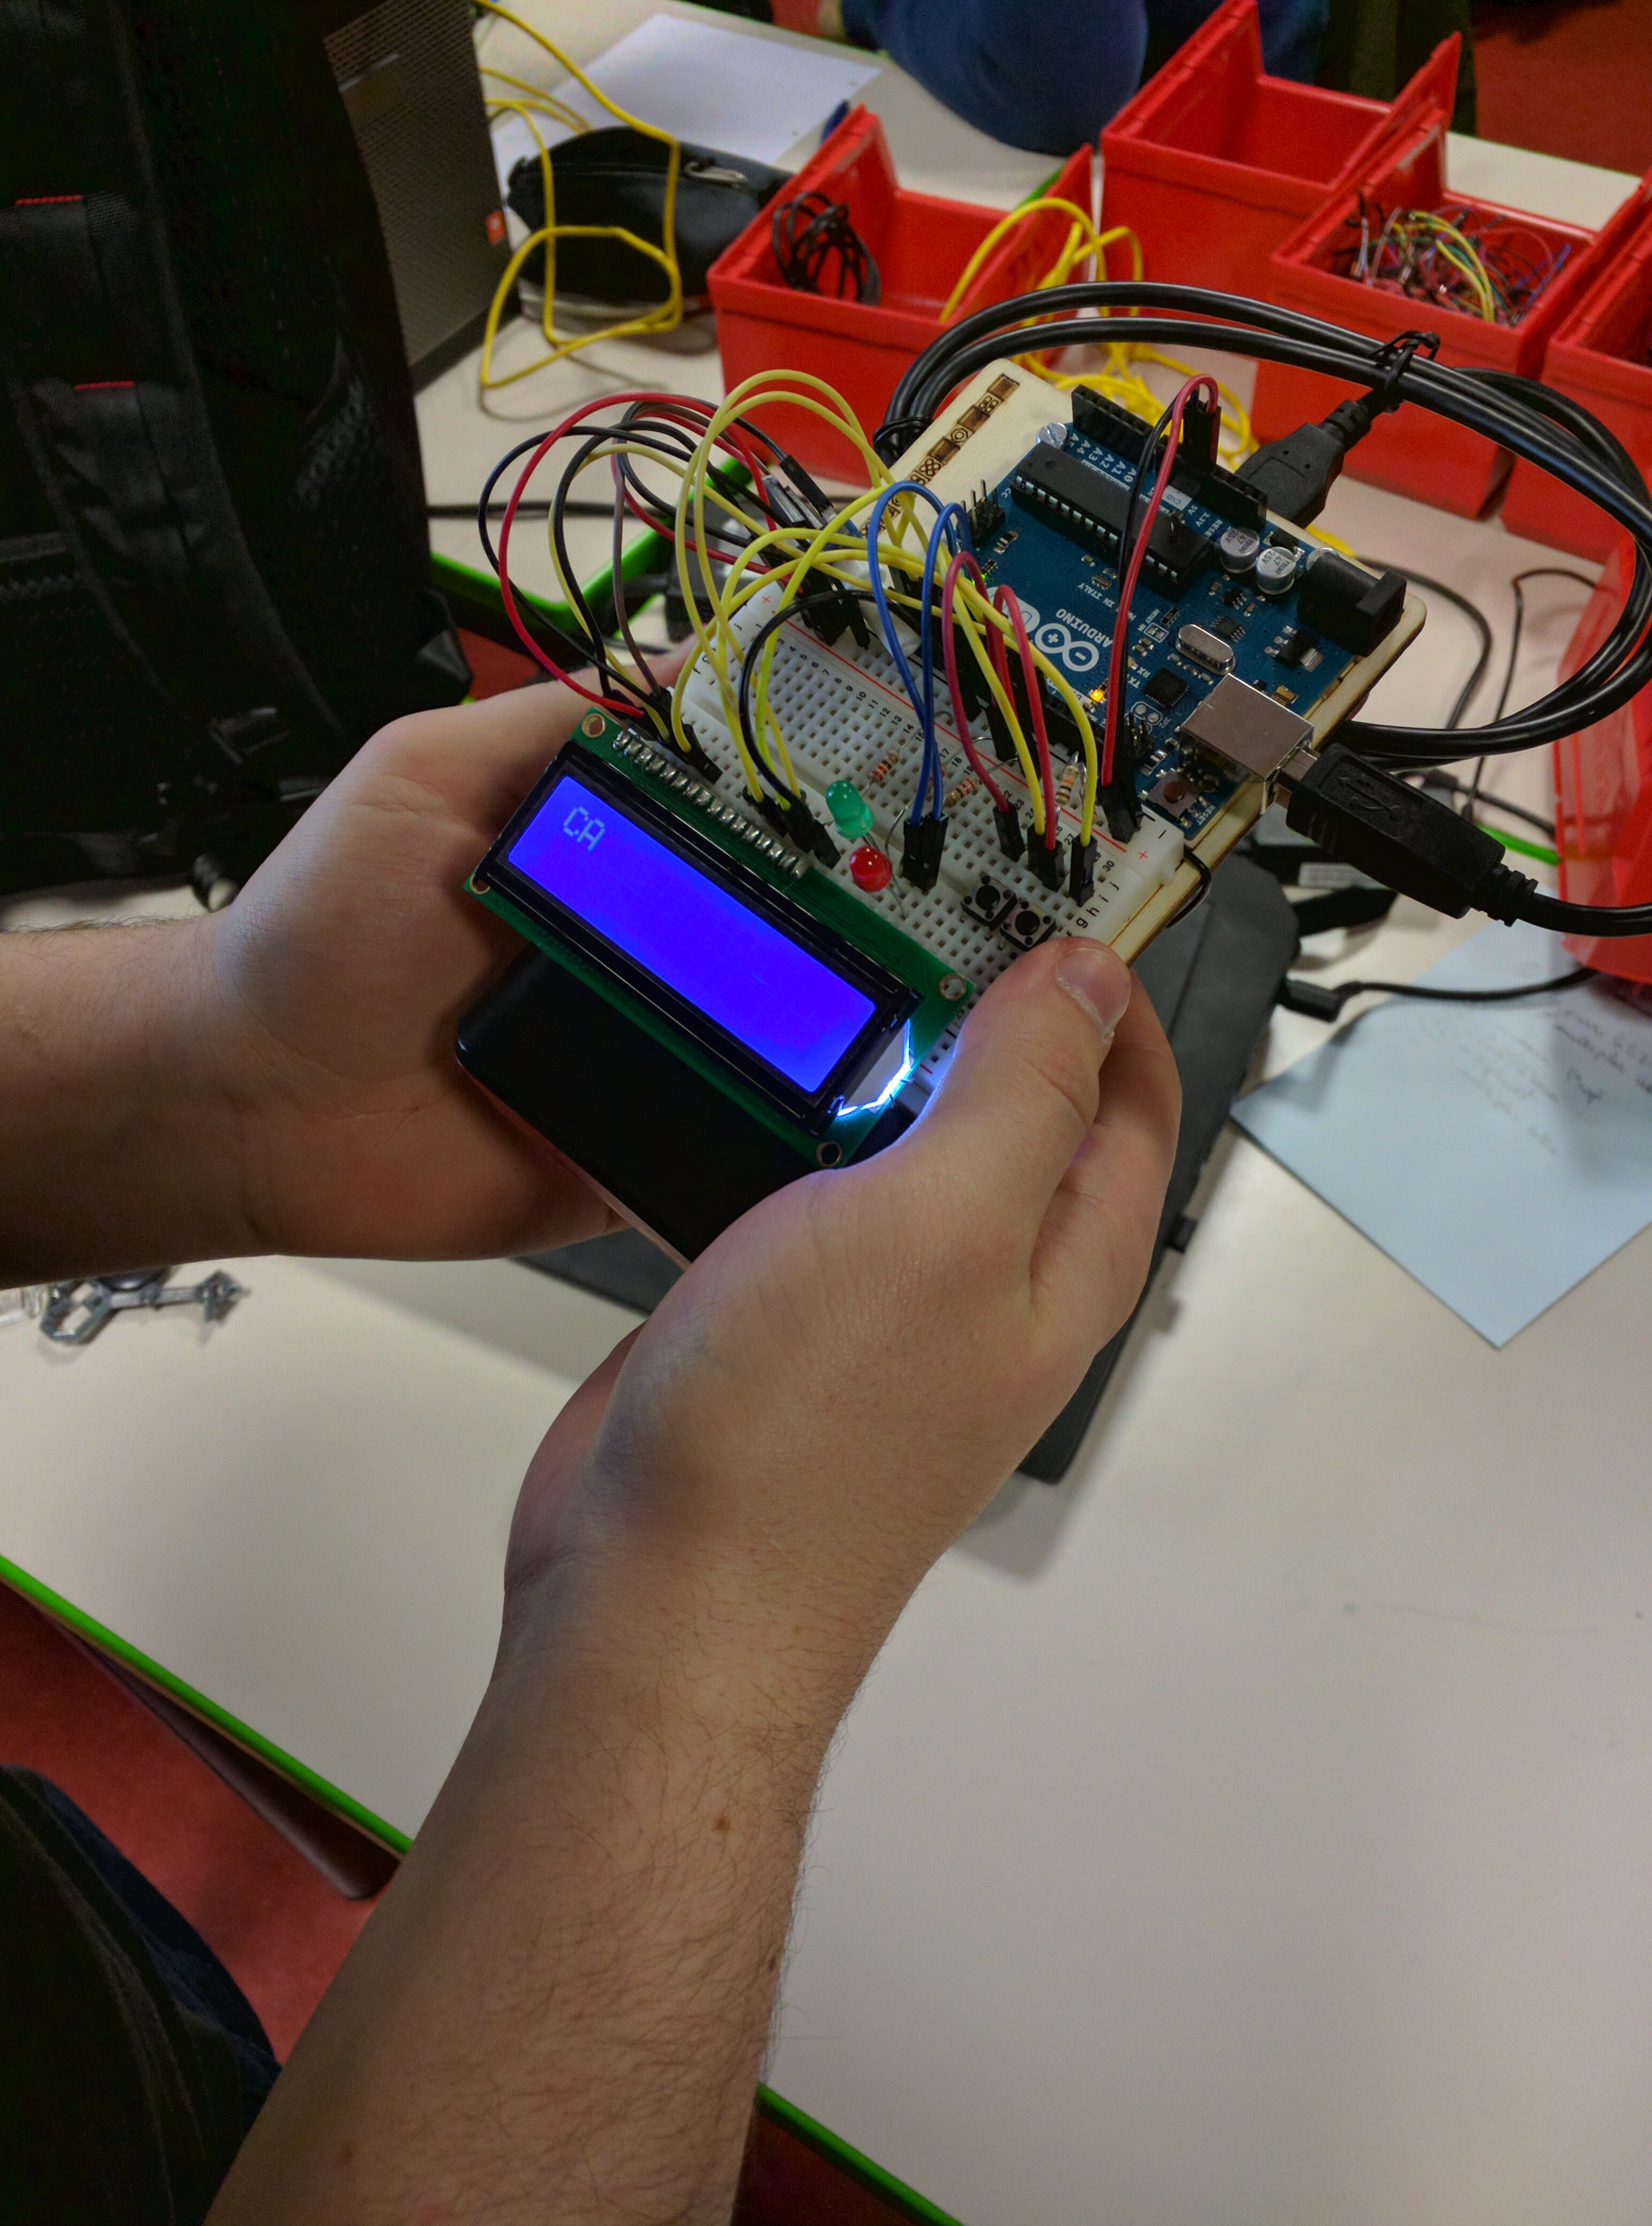
\includegraphics[width=8cm]{2.jpg}}
      \hspace{2mm}
      \subfloat[Partie de Mastermind]{\label{4}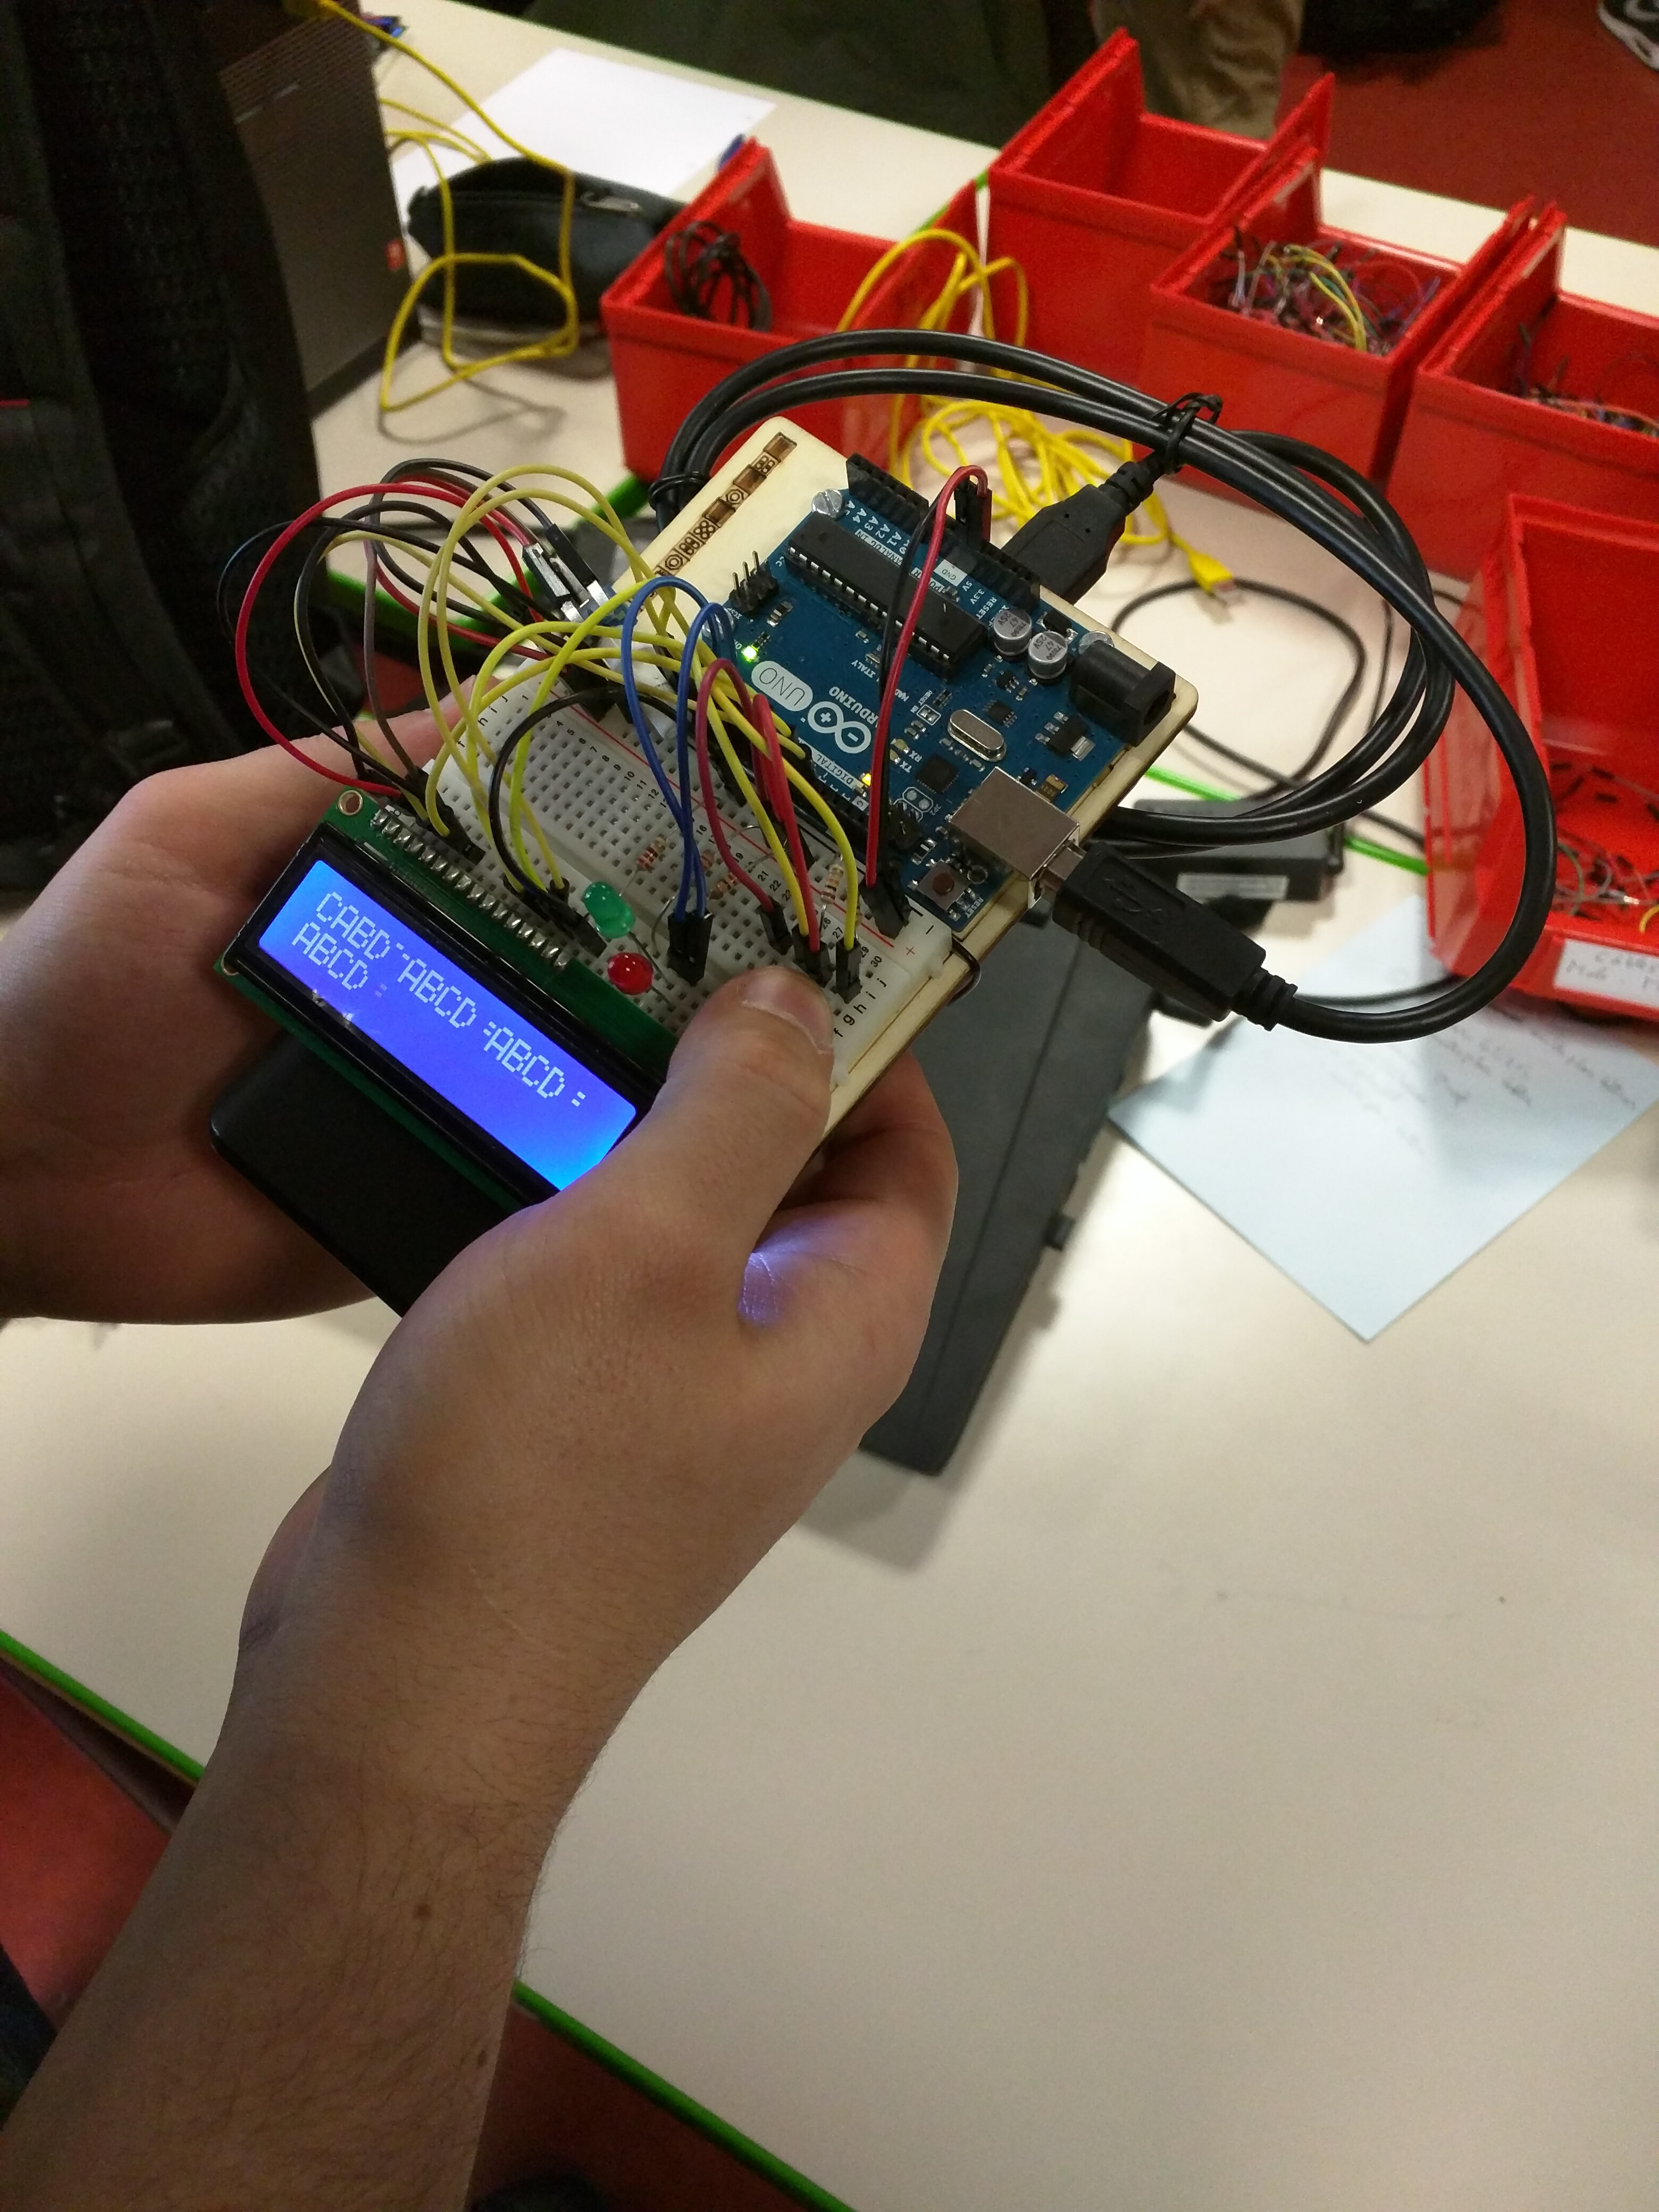
\includegraphics[width=8cm]{3.jpg}}
\end{figure}

\begin{figure}[h]
	\centering
		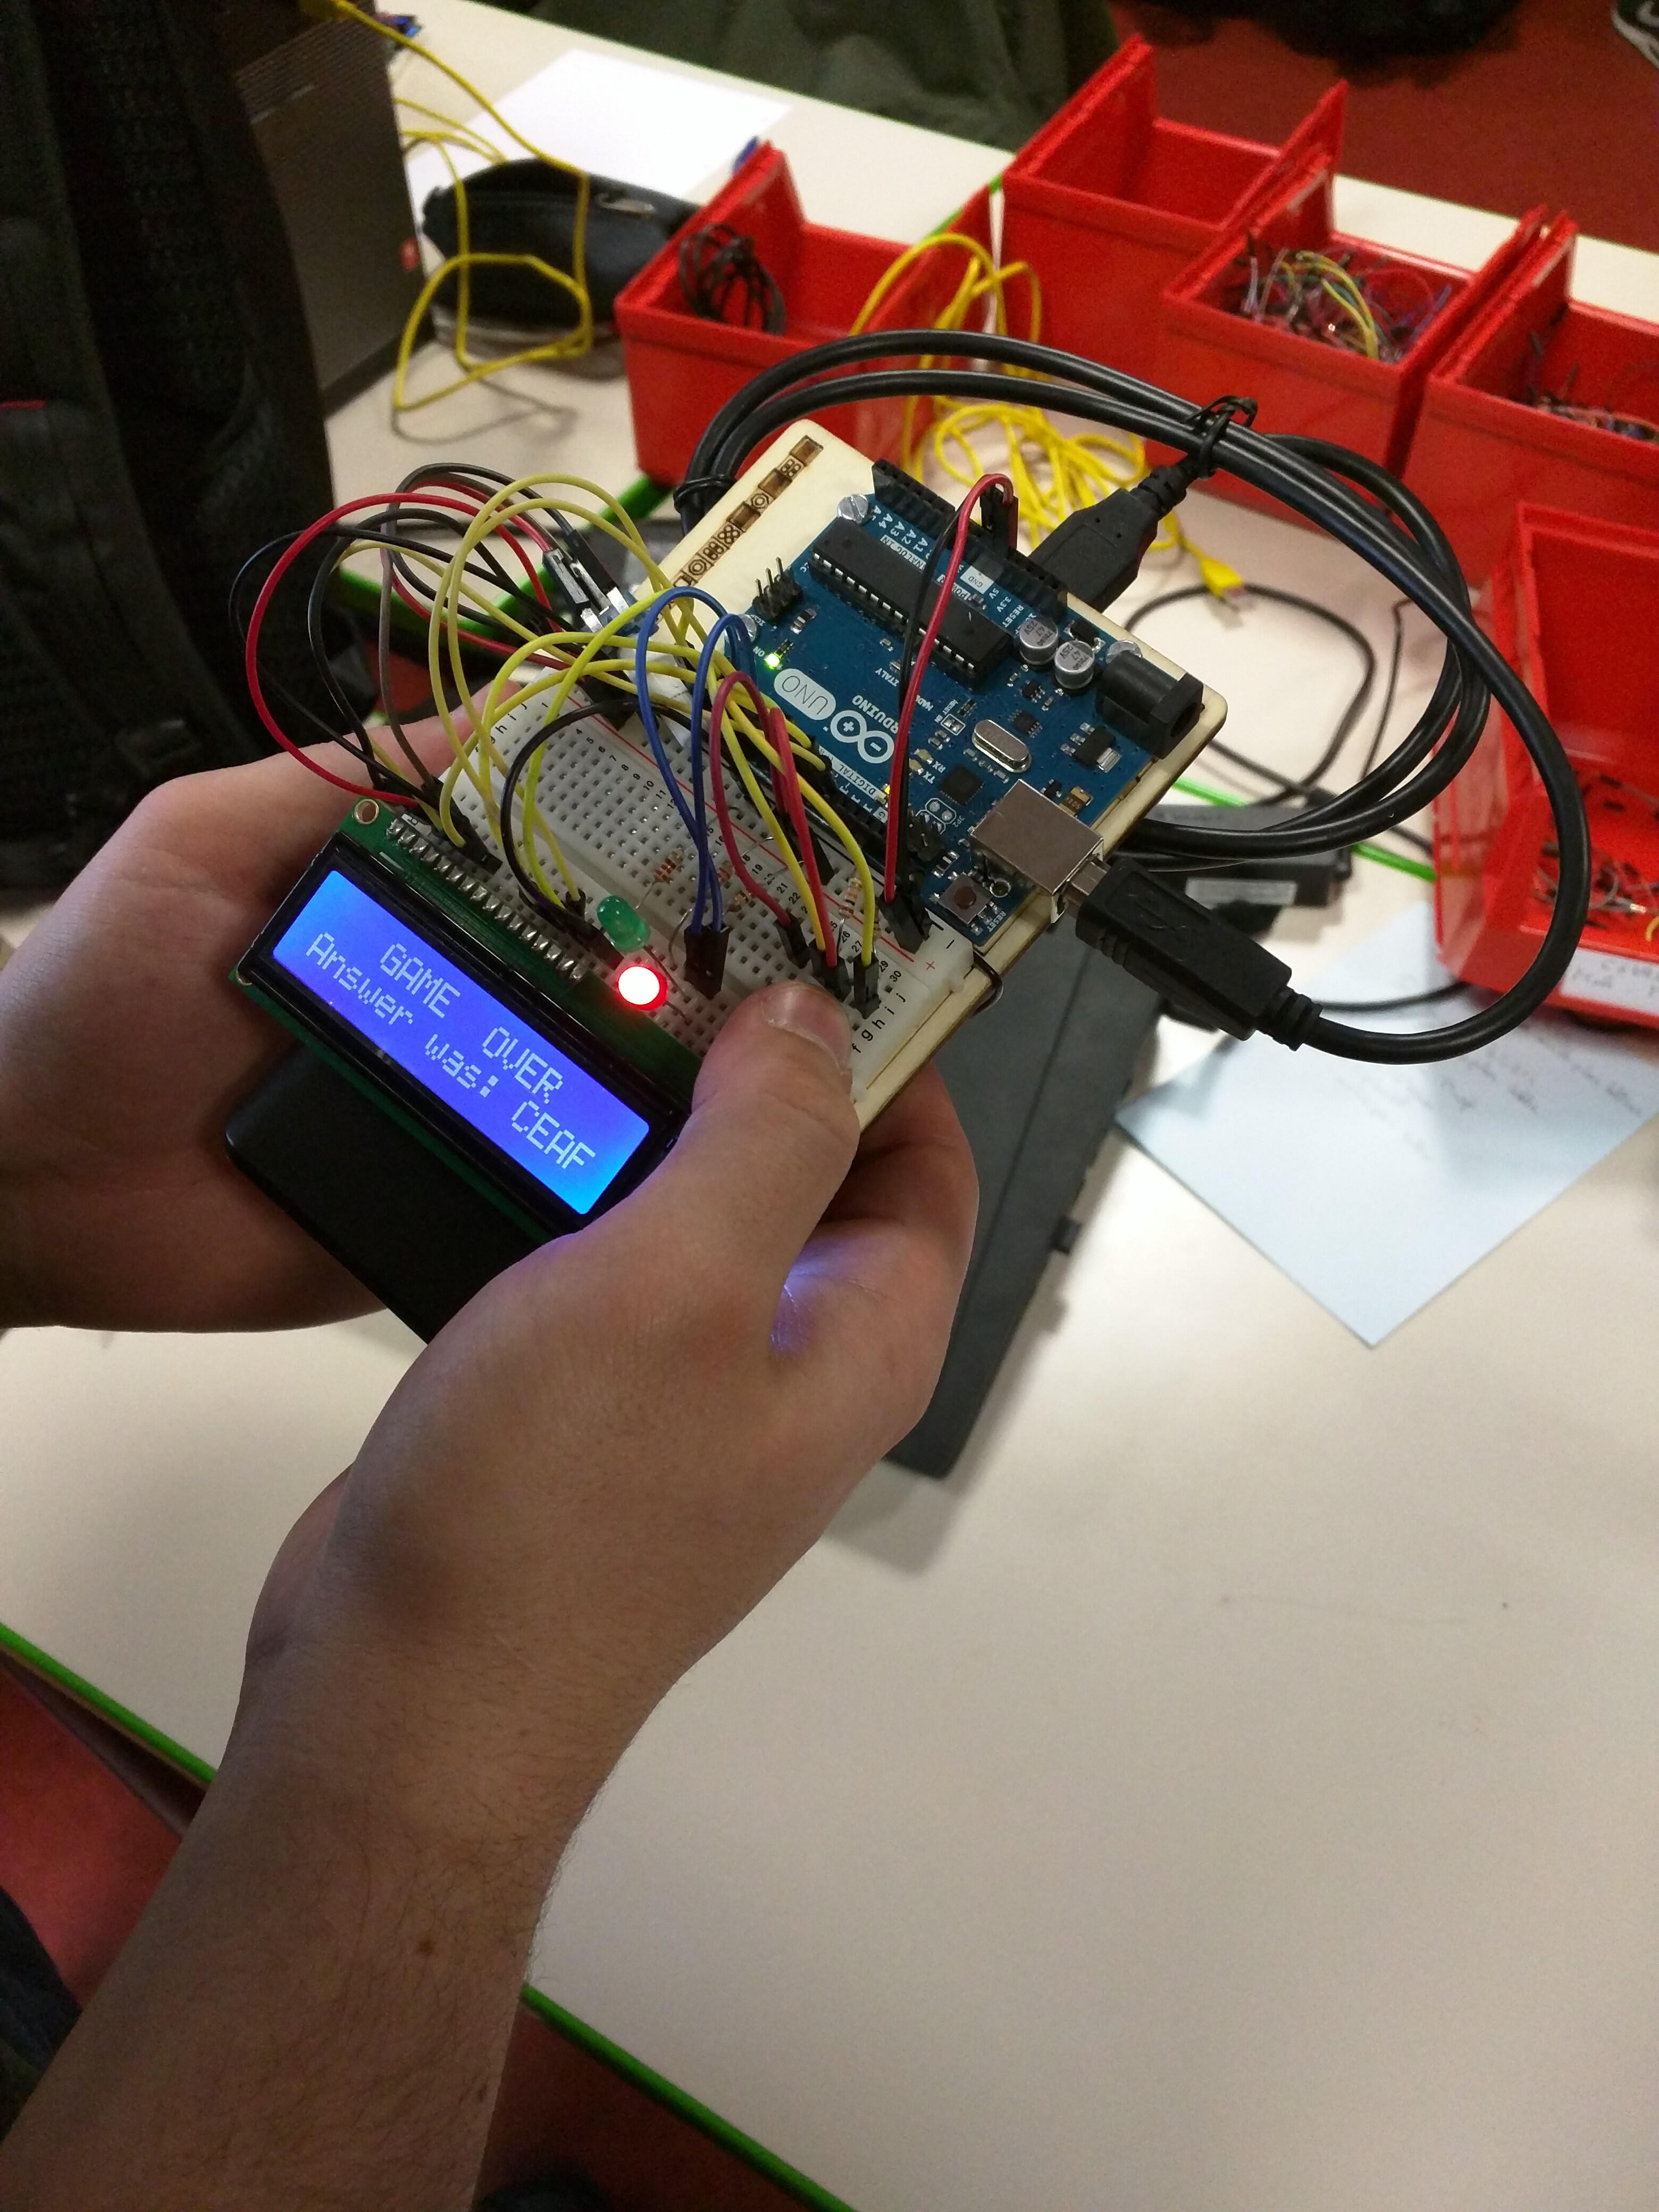
\includegraphics[width=18cm]{4.jpg}
        \caption{Fin de partie}
\end{figure}

\end{document}
